\documentclass[a4paper, 12pt]{article}		% general format

%%%% Charset
\usepackage{cmap}							% make PDF files searchable and copyable
\usepackage[utf8x]{inputenc}				% accept different input encodings
\usepackage[T2A]{fontenc}					% Russian font
\usepackage[russian]{babel}					% multilingual support (T2A)

%%%% Graphics
\usepackage[dvipsnames]{xcolor}			% driver-independent color extensions
\usepackage{graphicx}						% enhanced support for graphics
\usepackage{wrapfig}						% produces figures which text can flow around

%%%% Math
\usepackage{amsmath}						% American Mathematical Society (AMS) math facilities
\usepackage{amsfonts}						% fonts from the AMS
\usepackage{amssymb}						% additional math symbols

%%%% Typography (don't forget about cm-super)
\usepackage{microtype}						% subliminal refinements towards typographical perfection
\linespread{1.3}							% line spacing
\usepackage[left=2.5cm, right=1.5cm, top=2.5cm, bottom=2.5cm]{geometry}
\setlength{\parindent}{0pt}					% we don't want any paragraph indentation
\usepackage{parskip}						% add distance between paragraphs

%%%% Tables
\usepackage{tabularx}						% Normal tables
\usepackage{multirow}						% for tabular
\usepackage{hhline}							% for tabular


%%%% Other
\usepackage{url}							% verbatim with URL-sensitive line breaks
\usepackage{fancyvrb}						% verbatim with box
\setcounter{secnumdepth}{5}					%

%------------------------------------------------------------------------------
\usepackage{listings}						% typeset source code listings

% Настройки отображения кода
\lstset{
	% Настройки отображения
	breaklines=true,						% Перенос длинных строк
	basicstyle=\ttfamily\footnotesize,		% Шрифт для отображения кода
	frame=tblr								% draw a frame at all sides of the code block
	tabsize=2,								% tab space width
	showstringspaces=false,					% don't mark spaces in strings
	% Настройка отображения номеров строк. Если не нужно, то удалите весь блок
	numbers=left,							% Слева отображаются номера строк
	stepnumber=1,							% Каждую строку нумеровать
	numbersep=5pt,							% Отступ от кода
	numberstyle=\small\color{black},		% Стиль написания номеров строк
}

% Для настройки заголовка кода
\usepackage{caption}
\renewcommand{\lstlistingname}{Листинг} % Переименование Listings в нужное именование структуры
%------------------------------------------------------------------------------
\author{Семён Мартынов\\<semen.martynov@gmail.com>}
\title{WSO2 Enterprsie Mobility Manager}
\begin{document}
\maketitle
\tableofcontents{}

%------------------------------------------------------------------------------

\section{Введение}

Компания WSO2 разрабатывает ряд продуктов на общей платформе Carbon и собственную среду разработки -- WSO2 Developer Studio.

\section{WSO2 Enterprise Service Bus}

Enterprise Service Bus обеспечит интеграцию с корпоративными сервисами.

\section{WSO2 Enterprsie Mobility Manager}

\subsection{Требования к ПО}

От хоста, на котором будет запускаться Enterprsie Mobility Manager требуется иметь минимум 2ГБ свободной оперативной памяти (512МБ будут использованы для SOAP-сообщений, что достаточно для не большого количество пользователей но может создать проблемы при использовании в производственной среде). На винчестере потребуется порядка 1Гб, на считая маста, которое потребуется для хранения баз данных и лог-файлов.

Все продукты WSO2 на платформе Carbon запускаются и нормально работают на Oracle JDK 1.6.*/1.7.*. Версия JDK 1.8 на данный момент не поддерживается. Также разработчики не рекомендуют использовать OpenJDK.

В качестве базы данных можно использовать встроенное решение H2, которое обеспечивает потребности разработчиков и тестировщиков, но для развёртывания в реальной среде строит использовать полноценные СУБД -- Oracle, PostgreSQL, MySQL, MS SQL и т.д.

Для интеграции с существующей базой пользователей, поддерживается интеграция с OpenLDAP.

На клиентах (мобильных устройствах) на данный момент поддерживаются версии 6.0 - 7.0 для iOS, для Android:
\begin{itemize}
\item Ice Cream Sandwich (4.0.3 – 4.0.4)
\item Jelly Bean (4.1 – 4.3.1)
\item KitKat (4.4 – 4.4.4)
\item Lollipop (5.0)
\end{itemize}

Общий список програмномного обеспечения, которое может потребоваться, выглядят следующим образом:

\begin{tabular}{|c|c|c|}
\hline 
ПО & Версия & Примечание \\ 
\hline 
{Oracle JDK} & 1.6.24 или новее / 1.7 & Для запуска приложения \\ 
\hline 
MySQL & 5.6.* & База данных \\ 
\hline 
MySQL Connector/J & 5.1.* & Используется для свзи с БД \\ 
\hline 
Git & 1.8.* & Для доступа к репозиторию Android Agent \\ 
\hline 
Eclipse & Juno (4.2.1) или новее & Сборка клиентских приложений \\ 
\hline 
Android SDK & Уровень 8 - 17 & Сборка клиентских приложений \\ 
\hline 
Web-браузер & * & Для доступа к веб-интерфейсу \\ 
\hline 
Apache Ant & 1.7.0 или новее & Компиляция и сборка примеров приложений \\ 
\hline 
Apache Maven & 3.0.* & Сборка приложения из исходных кодов \\ 
\hline 
\end{tabular} 

\subsection{Подготовка хоста}

На основании предыдущего пункта, необходимо установить JDK1.7. Все действия будем проводить на Ubuntu 15.04 Server.

\begin{Verbatim}[frame=single]
user@wso2:~ cat /etc/lsb-release 
DISTRIB_ID=Ubuntu
DISTRIB_RELEASE=15.04
DISTRIB_CODENAME=vivid
DISTRIB_DESCRIPTION="Ubuntu 15.04"
\end{Verbatim}

Установку Java можно провести врчную, скачав исходники с сайта Oracle, но мы воспользуемся PPA, в котором эта процедура автоматизированна.

Для начала убедимся, что у нас уже не установлен OpenJDK.

\begin{Verbatim}[frame=single]
user@wso2:~ java -version
The program 'java' can be found in the following packages:
 * default-jre
 * gcj-4.9-jre-headless
 * openjdk-7-jre-headless
 * gcj-4.8-jre-headless
 * openjdk-6-jre-headless
 * openjdk-8-jre-headless
Try: sudo apt-get install <selected package>
\end{Verbatim}

Как видно выше, система ничего не знает о Java, значит можно продолжить выполнение установки. В противном случае потребовалось бы очистить систему от имеющихся пакетов командой (на самом деле в системе допустимо иметь несколько различных версий JDK и переключаться между ними, но мы сейчас это рассматривать не буедем).
\begin{Verbatim}[frame=single]
sudo apt-get remove openjdk*
\end{Verbatim}

Теперь можно перейти к добавлению PPA, содержащего JDK1.7. Для этого потребуется ввести следующие три команды (использование sudo требует ввода пароля суперпользователя).
\begin{Verbatim}[frame=single]
echo "deb http://ppa.launchpad.net/webupd8team/java/ubuntu vivid main" |\
                   sudo tee /etc/apt/sources.list.d/webupd8team-java.list
echo "deb-src http://ppa.launchpad.net/webupd8team/java/ubuntu vivid main" |\
                sudo tee -a /etc/apt/sources.list.d/webupd8team-java.list
sudo apt-key adv --keyserver hkp://keyserver.ubuntu.com:80\
                                                       --recv-keys EEA14886
\end{Verbatim}

Обновление списка пакетов и установка JDK.

\begin{Verbatim}[frame=single]
sudo apt-get update
sudo apt-get install oracle-java7-installer oracle-java7-set-default
\end{Verbatim}

В процессе установки потребуется принять лицензию Oracle.

После установки стоит убедиться в корректности работы JDK и наличию всех необходимых переменных окружения (для этого нужно завершить текущий сеанс и залогиниться по новой)

\begin{Verbatim}[frame=single]
user@wso2:~ java -version
java version "1.7.0_80"
Java(TM) SE Runtime Environment (build 1.7.0_80-b15)
Java HotSpot(TM) 64-Bit Server VM (build 24.80-b11, mixed mode)
user@wso2:~ javac -version
javac 1.7.0_80
user@wso2:~ env | grep -i java
DERBY_HOME=/usr/lib/jvm/java-7-oracle/db
PATH=/usr/local/sbin:/usr/local/bin:/usr/sbin:/usr/bin:/sbin:/bin:/usr/games:
/usr/local/games:/usr/lib/jvm/java-7-oracle/bin:/usr/lib/jvm/java-7-oracle/db
/bin:/usr/lib/jvm/java-7-oracle/jre/bin
JAVA_HOME=/usr/lib/jvm/java-7-oracle
J2SDKDIR=/usr/lib/jvm/java-7-oracle
J2REDIR=/usr/lib/jvm/java-7-oracle/jre
\end{Verbatim}

Система готова к работе с WSO2 Enterprsie Mobility Manager.

\subsection{Запуск Enterprsie Mobility Manager}

WSO2 Enterprsie Mobility Manager можно собрать из исходников либо воспользоваться готовыми бинарниками, распространяемыми разработчиками (размер архива 277MB).

\begin{Verbatim}[frame=single]
user@wso2:~ wget http://product-dist.wso2.com/products/enterprise-mobility-ma
nager/1.1.0/wso2emm-1.1.0.zip
\end{Verbatim}

Содержимосе архива нужно извлечь в директорию на винчестере, я предпочитаю для этого использовать opt.

\begin{Verbatim}[frame=single]
sudo unzip wso2emm-1.1.0.zip -d /opt
\end{Verbatim}

Для запуска воспользуемся скриптом из архива. Пока сделаем это от имени суперпользователя, позже разберёмся с правами более тонко.
\begin{Verbatim}[frame=single]
sudo -E sh /opt/wso2emm-1.1.0/bin/wso2server.sh
\end{Verbatim}

Когда система будет запущена, из браузера можно будет обратиться по адресу \url{https://192.168.124.185:9443/} (192.168.124.185 - мой IP виртуальной машины с WSO2 Enterprsie Mobility Manager) и получить доступ к панеле управления (рисунок 1). Имя пользователя и пароль по умолчанию admin.

\begin{figure}[h!]
\centering
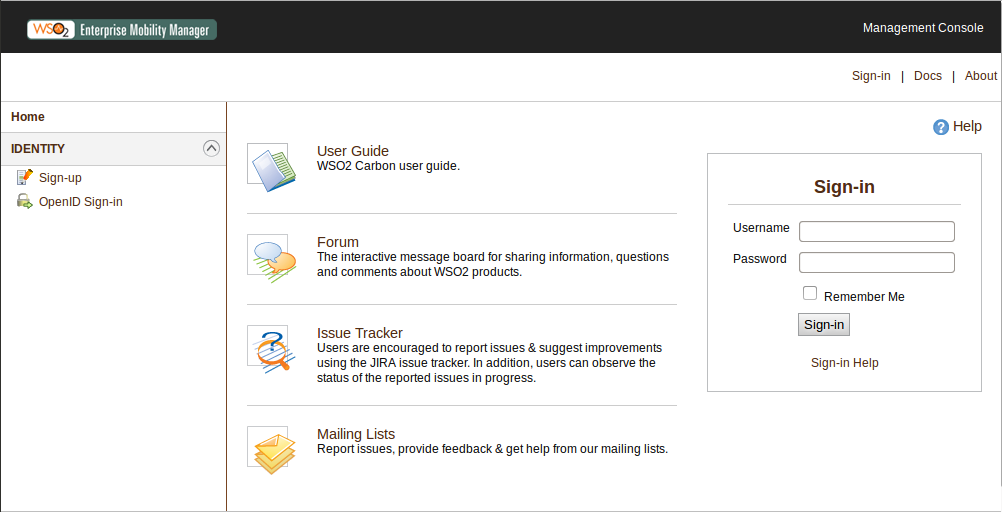
\includegraphics[scale=0.45]{res/EMM001}
\caption{Web-интерфейс EMM}
\end{figure}

\subsection{Автоматический запус EMM}

\subsection{Добавление устройств}

\section{WSO2 Developer Studio}

WSO2 Developer Studio представляет из себя Eclipse дополненный набором плагинов от WSO2. Установка среды разработки от WSO2 делается аналогично обычному Eclipse, нужно просто распаковать zip-архив..

Единственный важный момент о котором стоит помнить, это разнесение по портам различных продуктов WSO2 при их одновременном запуске. Для этой цели используется файла carbon.xml, а значения портов нужно прописать в теге <Offset>.

Подключение Enterprsie Mobility Manager к Developer Studio позволяет обеспечить запуск и просмотр логи сразу из среды программирования.



%------------------------------------------------------------------------------

\end{document}